% !TeX root = ../../Book3.tex
% 纲要标题：### 7.4 割迹与刚性
% 纲要位置：几何学计划纲要.md，第 2384 行。
% 正文状态：初稿；尚未正式审核。

% 纲要内容开始
% 
% * 割迹之外的光滑结论
% * 支撑函数及屏障解释
% * 分布意义下的 Laplace 比较
% * 等号传播及局部空间形式
% 
% ---
% 
% 纲要内容结束

\section{割迹与刚性}
\label{g3:sec:0704}

在割迹上，同一点可能由不同的最短线到达，距离函数因而出现折角；即使最短线唯一，指数映射也可能退化。前面的逐点 Hessian 公式不能直接在这些点取值。要保留比较结论，可以在待考察点上方放置光滑支撑函数，也可以把不等式与非负测试函数配对。本节分别建立这两种解释，并说明等号怎样从一条射线传播到整个法球。

\subsection{割迹之外的光滑结论}
\label{g3:subsec:0704:01}

设 \((M,g)\) 连通、完备、无边界，\(p\in M\)。沿用第二章的割时 \(c_p(u)\) 和开射线区域
\[
	\mathcal D_p=\{0\}\cup\{tu:u\in S_pM,\ 0<t<c_p(u)\}.
\]
\cref{g3:prop:distance-smooth-regular}已把第二章的集合双射加强为微分同胚：\(\exp_p:\mathcal D_p\to M\setminus\operatorname{Cut}(p)\)。特别地，\(\mathcal D_p\) 开，割迹闭，且 \(r=d(p,\cdot)\) 在 \(M\setminus(\{p\}\cup\operatorname{Cut}(p))\) 上光滑。这既给出前面比较定理的逐点适用区域，也使割时成为连续函数。

\begin{proposition}\label{g3:prop:cut-time-continuous}
	设 \((M,g)\) 为连通、完备、光滑无边界黎曼流形，\(p\in M\)。记 \(S_pM\) 为单位切球面、\(c_p\) 为割时函数。则 \(c_p:S_pM\to(0,\infty]\) 连续，其中趋于 \(\infty\) 按扩充实数的意义理解，并且
	\[
		\operatorname{inj}_g(p)=\inf_{u\in S_pM}c_p(u).
	\]
\end{proposition}
\begin{proof}
	第二章的\cref{g3:prop:cut-time-upper-semicontinuity}已经给出上半连续性。若 \(t<c_p(u)\)，则 \(tu\in\mathcal D_p\)。由其开性，充分接近 \(u\) 的 \(v\) 满足 \(tv\in\mathcal D_p\)，即 \(t<c_p(v)\)。对任意这样的 \(t\) 成立，故 \(c_p\) 下半连续。这也处理 \(c_p(u)=\infty\)：给定任意有限 \(t\)，邻近方向的割时最终都大于 \(t\)。

	记右侧下确界为 \(c_*\)。若 \(0<a<c_*\)，则 \(B_a(0)\subset\mathcal D_p\)，所以 \(\exp_p\) 在该球上为微分同胚，得到 \(\operatorname{inj}_g(p)\ge c_*\)。反向不等式正是\cref{g3:prop:compact-injectivity-lower-bound}在完备情形中的结论。两边允许同时为无穷。
\end{proof}

割迹在拓扑上可能相当复杂，但对体积积分有一个简单性质。下面的证明只需每条射线上恰有至多一个割时，不要求割迹是一张光滑超曲面。

\begin{proposition}\label{g3:prop:cut-locus-zero-volume}
	将法向空间沿线平行识别，径向 Jacobi 张量 \(A\) 满足 \(A''+\mathcal RA=0\)、\(A(0)=0\)、\(A'(0)=I\)，其中 \(\mathcal R=R(\cdot,\dot\gamma)\dot\gamma\)；在 \(A\) 可逆处记 \(S=A'A^{-1}\)、\(h=\operatorname{tr}S\)，\(I\) 为恒等算子。
	设 \((M^n,g)\) 为连通、完备、光滑无边界黎曼流形，\(n\ge2\)，\(p\in M\)。则 \(\operatorname{Cut}(p)\) 的黎曼体积为零。若 \(f\) 为非负可测函数，或为关于黎曼体积可积的函数，则
	\begin{equation}\label{g3:eq:polar-cut-integration}
		\int_M f\,\mu_g
		=\int_{S_pM}\int_0^{c_p(u)}
		f(\exp_p(tu))\,\theta(t,u)\,\mathrm{d}t\,\mathrm{d}\sigma(u),
	\end{equation}
	其中 \(\mathrm{d}\sigma\) 为单位切球面的标准面积密度，\(\theta(t,u)=\det A_u(t)>0\) 为径向 Jacobi 张量的行列式。
\end{proposition}
\begin{proof}
	在 \(S_pM\times(0,\infty)\) 中考虑有限割时的图
	\[
		\Gamma_p=\{(u,t):t=c_p(u)<\infty\}.
	\]
	连续性使这个集合可测；每条竖直纤维与它相交于至多一个点。对球面的有限坐标覆盖及有界时间区间使用 Fubini 定理，得 \(\Gamma_p\) 的 \(n\) 维乘积测度为零。映射 \(F(u,t)=\exp_p(tu)\) 光滑。在源、靶的相对紧坐标片内，其导数有界，因此为 Lipschitz 映射。这样的同维映射把零测集映成零测集：用总体积任意小的立方体覆盖原集，每个像可被边长至多为原边长固定倍数的立方体覆盖，即得所需外测度估计。取可数坐标覆盖，便知 \(F(\Gamma_p)=\operatorname{Cut}(p)\) 零测。

	在 \(0<t<c_p(u)\) 上，\(F\) 是到割迹补集去掉 \(p\) 的微分同胚。角向初始变化 \(w\in u^\perp\) 对应 \(J_w(0)=0\)、\(J_w'(0)=w\) 的 Jacobi 场，故角向微分为 \(A_u(t)w\)。径向微分为单位向量 \(T\)，由 Gauss 引理与所有角向微分正交。因此体积密度为
	\[
		F^*\mu_g=|\det A_u(t)|\,\mathrm{d}t\,\mathrm{d}\sigma(u).
	\]
	因 \(A_u(t)=tI+O(t^3)\)，行列式在起点附近为正；割时前没有共轭点，故其间不经过零，绝对值可去掉。坐标换元给出式\eqref{g3:eq:polar-cut-integration}，零测的割迹和单点 \(p\) 不影响体积积分。非负函数用单调收敛拼合，可积函数再分解正负部分。
\end{proof}

这里的零测结论允许计算普通体积积分；它不允许在分布导数中删除割迹。函数沿一个零测超曲面的导数跳跃，仍能产生集中在该处的测度。后面的分部积分会直接显示这一项的符号。

\subsection{支撑函数及屏障解释}
\label{g3:subsec:0704:02}

最短线的一个内部点可以替代原基点。这样得到的距离加上已经走过的长度，总在原距离上方；关键是新距离在终点确实光滑。

\begin{lemma}\label{g3:lem:shifted-distance-smooth}
	设 \((M,g)\) 为连通、完备、光滑无边界黎曼流形，\(\gamma:[0,\ell]\to M\) 是从 \(p\) 到 \(q\ne p\) 的单位速最短测地线。对任意 \(0<\varepsilon<\ell\)，记 \(r=d(p,\cdot)\)，令 \(p_\varepsilon=\gamma(\varepsilon)\)。则 \(q\notin\operatorname{Cut}(p_\varepsilon)\)，且
	\begin{equation}\label{g3:eq:shifted-distance-support}
		r_\varepsilon(x)=\varepsilon+d(p_\varepsilon,x)
	\end{equation}
	在 \(q\) 的某邻域内光滑，满足 \(r_\varepsilon\ge r\)、\(r_\varepsilon(q)=r(q)\) 及 \(\nabla r_\varepsilon(q)=\dot\gamma(\ell)\)。
\end{lemma}
\begin{proof}
	若存在另一条从 \(p_\varepsilon\) 到 \(q\) 的最短线，将它与 \(\gamma|_{[0,\varepsilon]}\) 拼接，长度仍为 \(\ell=d(p,q)\)。\cref{g3:lem:corner-shortening}迫使拼接处的速度相同；测地线初值唯一性便使两条后段相同。因此从 \(p_\varepsilon\) 到 \(q\) 的最短线唯一。

	再排除该段两端共轭。若存在非零 Jacobi 场 \(J\)，满足 \(J(\varepsilon)=J(\ell)=0\)，把它在 \([0,\varepsilon]\) 上补成零场，得连续分段光滑场 \(V\)。Jacobi 方程与分部积分给出 \(I_{[0,\ell]}(V,V)=0\)。整段最短，故它在相同时间区间内也使能量最小：任意竞争曲线 \(c\) 满足 \(E(c)\ge\operatorname{Len}(c)^2/(2\ell)\ge\ell/2\)。第二变分因而说明 \(I_{[0,\ell]}\) 半正定。于是对任意固定端点场 \(W\)，将 \(I(V+sW)\ge0\) 分别用于正负小数 \(s\)，得 \(I(V,W)=0\)。由\cref{g3:prop:index-form-kernel}，\(V\) 是整个区间上的光滑 Jacobi 场；它在一个非空区间恒为零，初值唯一性迫使它恒为零，与 \(J\ne0\) 矛盾。

	这条后段最短、唯一且无端点共轭，\cref{g3:thm:cut-point-alternative}遂排除 \(q\) 是 \(p_\varepsilon\) 的割点。距离的光滑性与梯度公式由\cref{g3:prop:distance-smooth-regular}得到。最后，三角不等式给出
	\[
		d(p,x)\le d(p,p_\varepsilon)+d(p_\varepsilon,x)=r_\varepsilon(x),
	\]
	而在 \(q\) 处，最短线的可加性使等号成立。
\end{proof}

\begin{figure}[htbp]
	\centering
	% !TeX root = ../Book3.tex
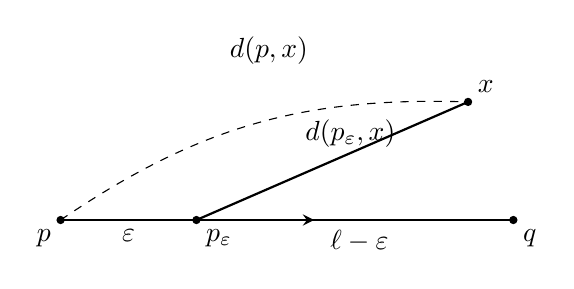
\begin{tikzpicture}[x=1.15cm,y=1cm,>=stealth]
	\coordinate (p) at (0,0);
	\coordinate (e) at (1.5,0);
	\coordinate (q) at (5,0);
	\coordinate (x) at (4.5,1.5);
	\draw[thick] (p)--(q);
	\draw[thick,->] (1.9,0)--(2.8,0);
	\draw[dashed] (p) to[bend left=18] (x);
	\draw[thick] (e)--(x);
	\node[above] at (2.3,1.85) {\(d(p,x)\)};
	\node[above,sloped] at (3.2,.8) {\(d(p_\varepsilon,x)\)};
	\node[below] at (.75,0) {\(\varepsilon\)};
	\node[below] at (3.3,0) {\(\ell-\varepsilon\)};
	\foreach \a in {p,e,q,x} {\fill (\a) circle (1.5pt);}
	\node[below left] at (p) {\(p\)};
	\node[below right] at (e) {\(p_\varepsilon\)};
	\node[below right] at (q) {\(q\)};
	\node[above right] at (x) {\(x\)};
\end{tikzpicture}

	\caption[移动基点构造距离的上支撑]{沿一条最短线把基点从 \(p\) 移到 \(p_\varepsilon\)。从 \(p\) 经 \(p_\varepsilon\) 到 \(x\) 的路线给出 \(r(x)\le\varepsilon+d(p_\varepsilon,x)\)，在 \(q\) 处取等号。图中的直线和弧线仅示意连接关系。}
	\label{g3:fig:distance-support}
\end{figure}

为准确说明“在割点仍成立”，暂记 \(L=\operatorname{div}\operatorname{grad}=-\Delta\)。若连续函数 \(f\) 在 \(q\) 附近满足：对每个 \(\eta>0\)，都有光滑函数 \(h\ge f\)，使 \(h(q)=f(q)\) 且 \(Lh(q)\le b+\eta\)，就称 \(Lf(q)\le b\) 在\term[shangzhicheng yiyi]{上支撑意义}[upper support sense]下成立，也称为相应的\term[pingzhang yiyi]{屏障意义}[barrier sense]。Hessian 的上支撑比较类似定义，以双线性型不等式 \(\operatorname{Hess}h(q)\le B+\eta g_q\) 代替迹不等式。支撑函数只需在 \(q\) 的一个邻域定义，邻域可以随 \(\eta\) 改变。

\begin{theorem}\label{g3:thm:distance-barrier-comparison}
	记 \(L=\operatorname{div}_g\operatorname{grad}_g\)、\(\Delta=-L\)，即采用非负 Laplace 算子约定。
	对给定 \(k\in\mathbb R\)，记 \(s_k\) 为满足 \(s_k''+ks_k=0\)、\(s_k(0)=0\)、\(s_k'(0)=1\) 的模型函数，\(b_k=\pi/\sqrt k\)（\(k>0\)）或 \(b_k=\infty\)（\(k\le0\)），\(\operatorname{ct}_k=s_k'/s_k\) 于 \((0,b_k)\)。
	设 \((M^n,g)\) 连通、完备、光滑且无边界，\(n\ge2\)，\(p\in M\)，\(r=d(p,\cdot)\)，\(k\in\mathbb R\)。若 \(\operatorname{Ric}\ge(n-1)kg\)，则在 \(0<r(q)<b_k\) 的每一点，包括割点，
	\[
		Lr(q)\le(n-1)\operatorname{ct}_k(r(q))
	\]
	在上支撑意义下成立；按本书符号，这就是相应的 \(\Delta r\ge-(n-1)\operatorname{ct}_k(r)\) 屏障估计。若更强地有截面曲率 \(K\ge k\)，选任一从 \(p\) 到 \(q\) 的单位速最短线的末速度 \(v\)，还得到上支撑意义下
	\[
		\operatorname{Hess}r(q)\le\operatorname{ct}_k(r(q))
		\bigl(g_q-v^\flat\otimes v^\flat\bigr).
	\]
\end{theorem}
\begin{proof}
	记 \(\ell=r(q)\)，应用上一引理。\(q\) 距新基点 \(p_\varepsilon\) 为 \(\ell-\varepsilon\)，且在其割迹之外。\cref{g3:thm:laplacian-comparison}给出
	\[
		Lr_\varepsilon(q)\le(n-1)\operatorname{ct}_k(\ell-\varepsilon).
	\]
	因为 \(0<\ell<b_k\)，右边在 \(\varepsilon\downarrow0\) 时趋于 \((n-1)\operatorname{ct}_k(\ell)\)。对给定 \(\eta>0\) 选足够小的 \(\varepsilon\)，即可得到定义要求的上支撑函数。截面曲率下界时，\cref{g3:thm:hessian-comparison}同样给出
	\[
		\operatorname{Hess}r_\varepsilon(q)
		\le\operatorname{ct}_k(\ell-\varepsilon)
		\bigl(g_q-v^\flat\otimes v^\flat\bigr).
	\]
	张量 \(g_q-v^\flat\otimes v^\flat\) 的算子范数为1，故系数的收敛也给出任意小的 \(\eta g_q\) 误差。
\end{proof}

这个构造在 \(\Delta=-L\) 的约定下仍使用距离的上支撑，而支撑函数的 \(\Delta\) 满足下界。它也给出一个便于辨认方向的测试：若光滑 \(\psi\le r\) 在 \(q\) 与 \(r\) 接触，则 \(\psi\le r_\varepsilon\) 且接触值相同，故 \(L\psi(q)\le Lr_\varepsilon(q)\)；取极限得到同一个上界。相反，截面曲率上界所给的光滑区域 Hessian 下界一般不能穿过割迹，因为割迹处的折角可能向下。

\subsection{分布意义下的 Laplace 比较}
\label{g3:subsec:0704:03}

屏障估计是逐点的接触陈述。积分论证还需要分布意义：把可能不光滑的函数与光滑紧支测试函数配对，将导数移到测试函数上。这里直接处理距离函数所需的情形。

\begin{lemma}\label{g3:lem:lipschitz-weak-gradient}
	记 \(L=\operatorname{div}_g\operatorname{grad}_g\)、\(\Delta=-L\)，即采用非负 Laplace 算子约定。
	设 \((M,g)\) 为光滑无边界黎曼流形，\(U\subset M\) 开，\(f:U\to\mathbb R\) 局部 Lipschitz，并在某个闭零测集 \(Z\) 之外光滑。则 \(f\) 的弱梯度由 \(U\setminus Z\) 上的经典梯度几乎处处给出。具体地，对任意光滑紧支向量场 \(X\) 及任意 \(\phi\in C_c^\infty(U)\)，
	\[
		\int_U f\operatorname{div}X\,\mu_g
		=-\int_U\langle\nabla f,X\rangle\,\mu_g,
		\qquad
		\int_U f\Delta\phi\,\mu_g
		=\int_U\langle\nabla f,\nabla\phi\rangle\,\mu_g.
	\]
\end{lemma}
\begin{proof}
	在相对紧坐标盒中，黎曼距离和坐标 Euclid 距离局部互相控制，因此 \(f\) 在坐标中也 Lipschitz。固定除 \(x^i\) 外的坐标，所得一元函数 Lipschitz，因而绝对连续：不交小区间上的函数增量绝对值之和至多为 Lipschitz 常数乘总长度。绝对连续函数的微积分基本定理给出该直线上的积分分部公式，其导数几乎处处存在且有界。

	由 Fubini，几乎每条坐标直线与 \(Z\) 相交于一维零测集。在其余点，刚才的一元导数等于光滑函数的 \(\partial_i f\)。再次用 Fubini，对紧支光滑 \(a\) 有
	\[
		\int f\,\partial_i a\,\mathrm{d}x
		=-\int (\partial_i f)a\,\mathrm{d}x.
	\]
	在此式中取 \(a=\sqrt{\det G}\,X^i\)，求和并使用第一章的散度坐标公式，便得坐标盒内的第一个等式。用有限个从属坐标片的光滑权重分解 \(X\)，额外的权重导数因和为1而相消，得到全局式。最后取 \(X=\nabla\phi\)，再用 \(\Delta=-\operatorname{div}\nabla\)，即得第二个等式。
\end{proof}

对局部可积的 \(f\)，定义分布 \(\Delta f\) 在测试函数 \(\phi\) 上的值为 \(\int f\Delta\phi\,\mu_g\)。若对每个非负 \(\phi\in C_c^\infty(U)\) 都有
\[
	\int_U f\Delta\phi\,\mu_g\ge\int_U b\phi\,\mu_g,
\]
就称 \(\Delta f\ge b\) 在\term[fenbu yiyi]{分布意义}[distributional sense]下成立。上一引理把这个定义转化为一阶导数的积分，因而可以用于1-Lipschitz 的距离函数。非负测试函数和不等式方向都是定义的一部分。

\begin{theorem}\label{g3:thm:distributional-laplacian-comparison}
	记 \(L=\operatorname{div}_g\operatorname{grad}_g\)、\(\Delta=-L\)，即采用非负 Laplace 算子约定。
	对给定 \(k\in\mathbb R\)，记 \(s_k\) 为满足 \(s_k''+ks_k=0\)、\(s_k(0)=0\)、\(s_k'(0)=1\) 的模型函数，\(b_k=\pi/\sqrt k\)（\(k>0\)）或 \(b_k=\infty\)（\(k\le0\)），\(\operatorname{ct}_k=s_k'/s_k\) 于 \((0,b_k)\)。
	设 \((M^n,g)\) 连通、完备、光滑且无边界，\(n\ge2\)，\(\operatorname{Ric}\ge(n-1)kg\)，\(p\in M\)。令 \(r=d(p,\cdot)\)、\(U_k=\{x:0<r(x)<b_k\}\)。则在 \(U_k\) 上
	\begin{equation}\label{g3:eq:distributional-laplacian-comparison}
		\Delta r\ge-(n-1)\operatorname{ct}_k(r)
	\end{equation}
	在分布意义下成立。等价地，对每个非负 \(\phi\in C_c^\infty(U_k)\)，
	\[
		\int_{U_k}\langle\nabla r,\nabla\phi\rangle\,\mu_g
		\ge-\int_{U_k}(n-1)\operatorname{ct}_k(r)\phi\,\mu_g.
	\]
\end{theorem}
\begin{proof}
	距离为1-Lipschitz，且在闭零测集 \(\{p\}\cup\operatorname{Cut}(p)\) 外光滑，故上一引理适用。取 \(0<a<R<b_k\)，使 \(\phi\) 的支集包含于 \(\{a<r<R\}\)，并把 \(R\) 取得严格大于支集上的最大距离。在式\eqref{g3:eq:polar-cut-integration}中写
	\[
		\Phi(t,u)=\phi(\exp_p(tu)),\qquad
		\tau(u)=\min\{c_p(u),R\}.
	\]
	当 \(0<t<c_p(u)\) 时，\(\nabla r=\partial_t\)，所以
	\[
		\int\langle\nabla r,\nabla\phi\rangle\,\mu_g
		=\int_{S_pM}\int_0^{\tau(u)}\partial_t\Phi\,\theta\,\mathrm{d}t\,\mathrm{d}\sigma(u).
	\]
	对每条射线作一元分部积分。起端项为零，因为 \(\Phi=0\) 于支集以前；末端在 \(\tau=R\) 时同样为零，在有限割时 \(\tau=c_p(u)<R\) 时为
	\(\Phi(c_p(u),u)\theta(c_p(u),u)\ge0\)。这里 \(A_u\) 光滑延拓至割时，\(\theta\) 从正值趋于非负值；若该端点共轭，行列式就是零。因此
	\begin{equation}\label{g3:eq:cut-boundary-flux}
		\int\langle\nabla r,\nabla\phi\rangle\,\mu_g
		=\mathcal B_p(\phi)-\int_{S_pM}\int_0^{\tau(u)}\Phi\,\partial_t\theta\,\mathrm{d}t\,\mathrm{d}\sigma,
		\qquad \mathcal B_p(\phi)\ge0.
	\end{equation}
	这些积分和端点极限可以按方向积分：在紧集 \(S_pM\times[0,R]\) 上，Jacobi 方程的光滑依赖给出 \(\theta\)、\(\partial_t\theta\) 的共同界，而 \(c_p\) 可测，测试函数又有紧支集。

	在割时之前，由\cref{g3:thm:riccati-trace-comparison}和行列式求导，
	\[
		\partial_t\theta=h\theta
		\le(n-1)\operatorname{ct}_k(t)\theta.
	\]
	由于 \(\Phi\ge0\)，将此式代入 \eqref{g3:eq:cut-boundary-flux}并保留非负末端项，得到
	\[
		\int\langle\nabla r,\nabla\phi\rangle\,\mu_g
		\ge-\int_{S_pM}\int_0^{\tau(u)}
		(n-1)\operatorname{ct}_k(t)\Phi\theta\,\mathrm{d}t\,\mathrm{d}\sigma.
	\]
	再用极坐标换元，右端就是所要求的积分。这个证明同时说明：割迹的贡献在 \(Lr\) 中为非正，在本书的 \(\Delta r\) 中为非负。
\end{proof}

常曲率的逐点公式不能照搬为越过割迹的分布等式。例如平坦圆柱上，距离在一条割线上由两支光滑函数取较小者；两支的一阶导数在那里发生向下跳跃。因此即使所有光滑点都满足模型等式，分布中仍会多出割线项。章末习题将计算这一项。

\subsection{等号传播及局部空间形式}
\label{g3:subsec:0704:04}

比较中的等号记录了证明里各个非负量同时消失。Rauch 比较的单一方向等号控制一条 Jacobi 场；Ricci 迹比较的等号还使径向形算子各特征值相同。只有在一族方向上获得这些信息，才会确定一个开区域的度量。

\begin{proposition}\label{g3:prop:radial-metric-evolution}
	将法向空间沿线平行识别，径向 Jacobi 张量 \(A\) 满足 \(A''+\mathcal RA=0\)、\(A(0)=0\)、\(A'(0)=I\)，其中 \(\mathcal R=R(\cdot,\dot\gamma)\dot\gamma\)；在 \(A\) 可逆处记 \(S=A'A^{-1}\)、\(h=\operatorname{tr}S\)，\(I\) 为恒等算子。
	沿所述测地线，\(T=\dot\gamma\)，\(R\) 表示 Levi-Civita 曲率，\(P\) 表示沿线平行移动，撇号表示协变导数。
	对给定 \(k\in\mathbb R\)，记 \(s_k\) 为满足 \(s_k''+ks_k=0\)、\(s_k(0)=0\)、\(s_k'(0)=1\) 的模型函数，\(b_k=\pi/\sqrt k\)（\(k>0\)）或 \(b_k=\infty\)（\(k\le0\)），\(\operatorname{ct}_k=s_k'/s_k\) 于 \((0,b_k)\)。
	设 \((M^n,g)\) 为光滑无边界黎曼流形，\(p\in M\)，且 \(\exp_p\) 在切球 \(B_R(0)\) 上为微分同胚。令 \(F(t,u)=\exp_p(tu)\)，\(0<t<R\)、\(u\in S_pM\)。则
	\[
		F^*g=\mathrm{d}t^2+G_t,
	\]
	其中 \(G_t\) 是单位切球面上的度量族。若沿每条射线有 \(S(t)=\operatorname{ct}_k(t)I\)，且 \(R\le b_k\)，则
	\begin{equation}\label{g3:eq:model-polar-metric-rigidity}
		G_t=s_k(t)^2g_{S_pM}.
	\end{equation}
\end{proposition}
\begin{proof}
	Gauss 引理给出径向与角向的正交分解。对 \(u^\perp=\mathrm{T}_uS_pM\) 中的 \(a,b\)，令 \(J_a,J_b\) 为对应角向 Jacobi 场，则
	\[
		G_t(a,b)=\langle J_a(t),J_b(t)\rangle.
	\]
	径向形算子满足 \(J_a'=SJ_a\)，故
	\[
		\partial_tG_t(a,b)
		=\langle SJ_a,J_b\rangle+\langle J_a,SJ_b\rangle.
	\]
	当 \(S=\operatorname{ct}_k I\) 时，右端为 \(2\operatorname{ct}_kG_t(a,b)\)，于是 \(\partial_t(s_k^{-2}G_t)=0\)。另一方面，\(J_a(t)=tP_ta+O(t^3)\)、\(s_k(t)/t\to1\)，因此 \(s_k(t)^{-2}G_t(a,b)\to\langle a,b\rangle\)。常数只能是单位切球面的标准度量，得到式\eqref{g3:eq:model-polar-metric-rigidity}。
\end{proof}

\begin{theorem}\label{g3:thm:laplacian-equality-local-space-form}
	记 \(L=\operatorname{div}_g\operatorname{grad}_g\)、\(\Delta=-L\)，即采用非负 Laplace 算子约定。
	对给定 \(k\in\mathbb R\)，记 \(s_k\) 为满足 \(s_k''+ks_k=0\)、\(s_k(0)=0\)、\(s_k'(0)=1\) 的模型函数，\(b_k=\pi/\sqrt k\)（\(k>0\)）或 \(b_k=\infty\)（\(k\le0\)），\(\operatorname{ct}_k=s_k'/s_k\) 于 \((0,b_k)\)。
	设 \((M^n,g)\) 连通、完备、光滑且无边界，\(n\ge2\)，\(\operatorname{Ric}\ge(n-1)kg\)，\(p\in M\)，\(r=d(p,\cdot)\)。设 \(0<R<\min\{\operatorname{inj}_g(p),b_k\}\)。若对每个 \(u\in S_pM\)，在 \(q=\exp_p(Ru)\) 处都有
	\[
		\Delta r(q)=-(n-1)\operatorname{ct}_k(R),
	\]
	则 \(B(p,R)\) 与常截面曲率 \(k\) 的标准模型中半径 \(R\) 的球等距，且等距可取为指定起点切空间线性等距所诱导的指数坐标对应。
\end{theorem}
\begin{proof}
	沿任意固定方向 \(u\)，所给等号就是 \(h(R)=(n-1)\operatorname{ct}_k(R)\)。由\cref{g3:prop:riccati-trace-rigidity}，该方向上全部 \(0<t\le R\) 满足 \(S=\operatorname{ct}_k I\)。其证明中的等号分别使 \(\operatorname{Ric}(T,T)=(n-1)k\) 和无迹部分 \(S-hI/(n-1)\) 为零；因此得到的是整个径向算子的结论。对所有方向应用上一命题，便有
	\[
		F^*g=\mathrm{d}t^2+s_k(t)^2g_{S_pM}.
	\]
	在标准常曲率模型上，\cref{g3:exm:constant-curvature-jacobi}给出同样的角向 Jacobi 场和同样的极坐标度量。任选两起点切空间间的线性等距，先在切球中对应向量，再分别使用指数映射，就得到穿孔球上的等距。该对应本身在中心光滑，其微分为所选线性等距，所以由度量的连续性，中心处也保持度量。\(R\) 小于两侧的指数单射半径，故该对应是整个球的微分同胚与等距。
\end{proof}

这里只需在整张半径 \(R\) 的测地球面上取得迹等号，就能沿各射线向内恢复整个球的度量。若只在一个方向取得等号，结论相应限于这一条射线；若只知道一支 Jacobi 场的长度达到 Rauch 等号，控制的方向还要更少。下一章将把径向密度的不等式沿方向积分，得到球体积比较，并继续分析整体几何受到的限制。
% 纲要条目排为编号小节标题，并进入目录与书签；说明段仍保留于纲要注释中。
